Se desea obtener, a partir del circuito de la figura \ref{2.0}, el valor de la resistencia $R_x$ para cumplir con la condición de amplitud. Además, se desea saber cuál es la frecuencia de oscilación del circuito. 

\begin{figure}[H]
\centering
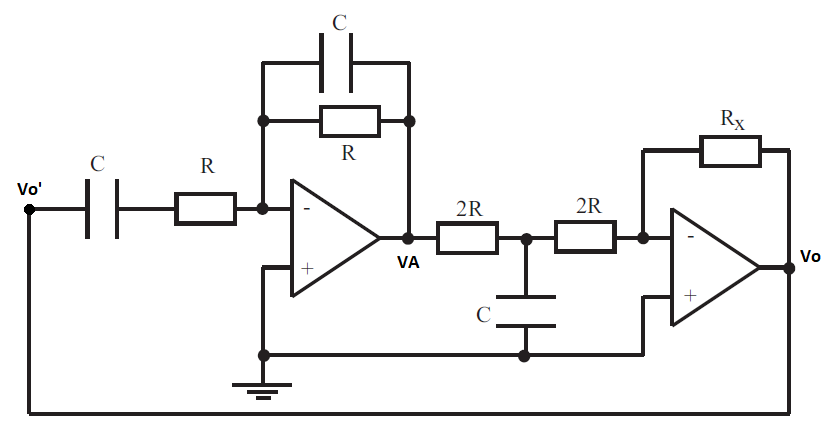
\includegraphics[width=0.6\linewidth]{images/circuito_1.png}
\caption{Circuito oscilador RC.}
\label{2.0}
\end{figure}

Debido a las características ideales de los amplificadores operacionales, se puede cortar el lazo cerrado justo en la rama entre los nodos $V_o'$ y $V_o$. De esta forma, el circuito de la figura \ref{2.0} queda como la figura \ref{2.1}, donde en esta última se observan los bloques correspondientes al amplificador $a(w_o)$ (color naranja) y la red selectiva de frecuencia $\beta (w_o)$ (color verde). Se aplica entonces un equivalente de Thevenin (color rojo) en el sitio indicado:

\begin{equation}
\label{eq:2.0}
\frac{V_A}{V_o'} = - \frac{Z_{R\parallel C}}{Z_{R-C}}= - \frac{\frac{R}{j wRC+1}}{\frac{j wRC+1}{j wC}} = - \frac{jwRC}{(jwRC+1)^2}
\end{equation}


\begin{figure}[H]
\centering
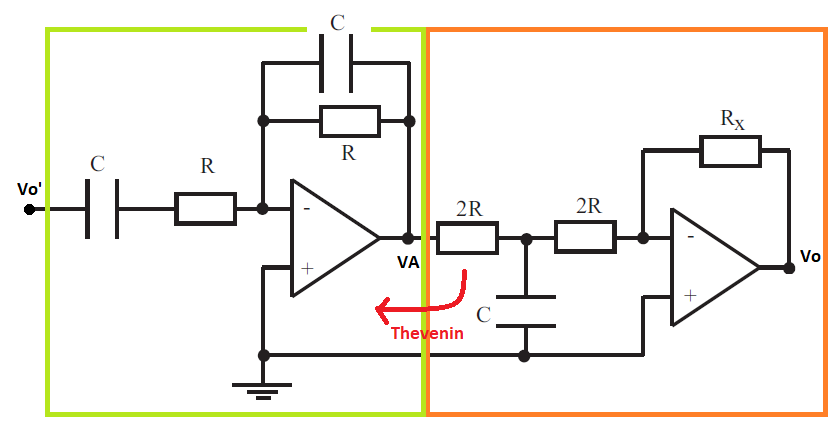
\includegraphics[width=0.6\linewidth]{images/circuito_1_1.png}
\caption{Circuito oscilador RC a lazo abierto.}
\label{2.1}
\end{figure}

Luego se vuelve a aplicar Thevenin pero esta vez en la entrada no inversora del amplificador operacional de $a(w_o)$. La impedancia que ve tal entrada es:

\begin{equation}
\label{eq:2.1}
Z_o = 2R + \frac{2R}{jwCR+1} = 4R\cdot \frac{(jwCR+1)}{(jw2CR+1)}
\end{equation}

Donde la fuente de thevenin correspondiente es, con el divisor resistivo $RC$ (configuración pasa-bajos):

\begin{equation}
\label{eq:2.2}
V_{th} = V_A \cdot \frac{1}{1+jwC2R}
\end{equation}

El circuito posee la forma como se observa en la figura \ref{2.2}.


\begin{figure}[H]
  	\centering
		 \begin{circuitikz}[european]
		 \draw
		  % El amplificador operacional
		  (0,0) node[op amp] (opamp) {} node[] {{\tiny Amp Op}}
		  % Las entradas
		  (opamp.-) node[circ] {} to[generic, l_=$Z_o$] ++(-2,0)
		  to[sinusoidal voltage source, l_=$V_{th}$] ++(0,-2) {} node[ground] 
		  ;
		  \draw
		  (opamp.+) -- ++(-0.5,0) -- ++(0,-1) node[ground] {} 
		  ;
		  % El lazo de realimentación
		  \draw
		  (opamp.-) -- ++(0,1)  to[R, l=$R_x$] ++(2,0)  -| (opamp.out) node[circ] {}
		  
		  % La salida
		  (opamp.out) -- ++(1,0) node[ocirc] {} node[right]{$V_o$}
		  ;
		\end{circuitikz}
    \caption[Circuito equivalente]{Circuito equivalente.}
    \label{2.2}
\end{figure}

La configuración del circuito equivalente de la figura anterior es conocida por lo que su función transferencia es, simplemente:

\begin{equation}
\label{eq:2.3}
\frac{V_o}{V_{th}} = - \frac{R_x}{Z_o}
\end{equation}

La ganancia de lazo abierto es:

\begin{equation}
\label{eq:2.4}
\frac{V_o}{V_o'} = \frac{V_o}{V_{th}} \cdot \frac{V_{th}}{V_A} \cdot \frac{V_A}{V_o'} = - \frac{R_x}{Z_o} \cdot \frac{1}{1+jwC2R} \cdot - \frac{jwRC}{(jwRC+1)^2}
\end{equation}

Trabajando algebraicamente, sabiendo que $Z_o$ posee la forma de la ecuación \ref{eq:2.1}, entonces:

\begin{equation}
\label{eq:2.5}
\frac{V_o}{V_o'} =R_x \cdot \frac{jwC}{4\cdot\{1-3\cdot (wCR)^2\} + 4j\cdot \{2wCR-(wCR)^3\}}
\end{equation}

La condición de fase establece que la fase de la transferencia de lazo abierto debe ser nula, por lo que, anulando la parte real del denominador de la expresión \ref{eq:2.5}, se elimina la parte imaginaria, por lo que el único valor de $w_o$ para el cual ocurre esto es, efectivamente, la frecuencia de oscilación:

\begin{equation}
\label{eq:2.6}
w_o = \frac{1}{\sqrt{3}\cdot RC}
\end{equation}

O mismo también:

\begin{equation}
\label{eq:2.7}
f_o = \frac{1}{2\pi \cdot \sqrt{3}\cdot RC}
\end{equation}

La expresión \ref{eq:2.5} posee la forma: 

\begin{equation}
\label{eq:2.8}
\frac{V_o}{V_o'} =R_x \cdot \frac{w_oC}{4\cdot \{2wCR-(wCR)^3\}}
\end{equation}

Pero la condición de amplitud establece que la transferencia de lazo abierto debe ser unitaria, por lo tanto, despejando se obtiene el valor de la resistencia $R_x$ para que el circuito oscile a una frecuencia $w_o$ (ecuación \ref{eq:2.6}):

\begin{equation}
\label{eq:2.9}
R_x = 4 \cdot \frac{\{2wCR-(wCR)^3\}}{w_oC} = \frac{32}{3} \cdot R
\end{equation}